\chapter{Listes}
\label{ch:listes}
Le type \mintinline{python}{list} permet de stocker des valeurs dans un ordre précis.
\begin{pyc}
	\begin{minted}{python}
		# on crée une liste avec 3 valeurs
		lst = ['bonjour', 3.14, True]
	\end{minted}
\end{pyc}
Une valeur de type \mintinline{python}{list} est itérable :
\begin{itemize}
	\item on peut accéder à un élément de la liste, par exemple \mintinline{python}{lst[0]} ;
	\item on peut parcourir une liste.
\end{itemize}

Pour accéder à un élement d'une liste situé à un endroit précis, on doit connaître son \textit{indice} : le premier élément d'une liste a l'indice zéro, le deuxième l'indice 1, \textit{et cætera}.

\begin{pyc}
	\begin{minted}{python}
		# on crée une liste avec 3 valeurs
		>>> lst = ['bonjour', 3.14, True]
		# premier élément : indice 0
		>>> lst[0]
		'bonjour'

		# deuxième élément
		>>> lst[1] 
		3.14
	\end{minted}
\end{pyc}

\section{Opérations de base}

\subsection{Créer une liste}

\begin{itemize}
	\item \mintinline{python}{lst = list()} crée une liste vide ;
	\item \mintinline{python}{lst = []} fait la même chose ;
	\item  \mintinline{python}{lst = ['a', 7, True]} crée une liste composée de 3 éléments.
\end{itemize}
Une liste peut contenir des éléments de plusieurs types mais en pratique on évite cela.


\subsection{Modifier un élément}
Le type \mintinline{python}{list} est \textit{mutable} : on peut changer un ou des éléments d'une liste \textit{sans changer la liste elle-même}.

\begin{pyc}
	\begin{minted}{python}
		>>> lst = [2, 3, 4, 1]
		# on change le deuxième élément
		>>> lst[1] = 10
		>>> lst
		[2, 10, 4, 1]
	\end{minted}
\end{pyc}
\subsection{Ajouter un élément en fin de liste}

On reprend l'exemple précédent

\begin{pyc}
	\begin{minted}{python}
		>>> lst.append(7) # ajoute 7 à la fin de la liste
		>>> lst
		[2, 10, 4, 1, 7]
	\end{minted}
\end{pyc}

\begin{remarque}
	\mintinline{python}{lst = lst + [7]} a le même effet  que \mintinline{python}{lst.append(7)} : on crée une « mini-liste » \mintinline{python}{[4]}, on concatène les 2 listes et on remet le résultat dans \mintinline{python}{lst}.\\
	En pratique la première méthode est la plus simple et aussi la plus rapide.
\end{remarque}

\subsection{Insérer un élément à une place donnée}

Pour une liste \mintinline{python}{lst} valant \mintinline{python}{[2, 10, 4, 1]}, si on veut insérer la valeur 5 à l'indice 1 on écrira :\\

\mintinline{python}{lst.insert(1, 5)} \\

et \mintinline{python}{lst} vaudra \mintinline{python}{[2, 5, 10, 4, 1]}\\

La syntaxe est \mintinline{python}{lst.insert(indice, valeur)}
\subsection{Retirer un élément à une position donnée}
Si une liste \mintinline{python}{lst} a pour valeur \mintinline{python}{[3 ,7, 1]} et qu'on veut supprimer son deuxième élément alors on écrit :\\

\mintinline{python}{del lst[1]}\\

Ensuite, \mintinline{python}{lst} aura la valeur \mintinline{python}{[3,1]}.

\subsection{Retirer une valeur précise}
Pour retirer une valeur \textit{qui appartient à une liste} on procède ainsi :\\

Si \mintinline{python}{lst} a la valeur \mintinline{python}{[1, 2, 5, 4, 2, 3]} alors l'instruction \\

\mintinline{python}{lst.remove(2)}\\

Supprime la \textit{première occurrence} de \mintinline{python}{2} dans \mintinline{python}{lst}.\\
Après cela, \mintinline{python}{lst} a la valeur \mintinline{python}{[1, 5, 4, 2, 3]}.


\subsection{Concaténer des listes}
On peut procéder de 2 manières :
\begin{itemize}
	\item \mintinline{python}{lst1.extend(lst2)} ajoute les éléments de la liste \mintinline{python}{lst2} à la fin de \mintinline{python}{lst1} ;
	\item \mintinline{python}{lst1 = lst1 + lst2} crée une liste avec les éléments de \mintinline{python}{lst1} et ceux de \mintinline{python}{lst2}, puis replace le résultat dans \mintinline{python}{lst1}.
\end{itemize}
En pratique la première méthode est plus rapide.


\subsection{Longueur d'une liste}
La fonction \mintinline{python}{len}
\begin{itemize}
	\item prend en entrée une liste \mintinline{python}{lst} ;
	\item renvoie la longueur de cette liste.
\end{itemize}

Ainsi \mintinline{python}{len([2, 3, 4])} vaut 3.

\subsection{Divers}
\mintinline{python}{lst.sort()} trie la liste dans l'ordre croissant.\\

\mintinline{python}{lst.reverse()} met les éléments dans l'ordre inverse.

\section{Opérations avancées}


\subsection{Copier une liste (mauvaise méthode)}
\begin{pyc}
	\begin{minted}{python}
>>> lst1 = [5, 6, 8]
>>> lst2 = lst1
>>> lst1[0] = 10
>>> lst1
[10, 6, 8]

>>> lst2
[10, 6, 8]  # problème : lst2[0] a changé aussi !
\end{minted}
\end{pyc}

Ce comportement « étrange » vient du fait que le type \mintinline{python}{list} est \textit{mutable}. Nous allons expliquer cela plus tard dans ce chapitre.

\subsection{Copier une liste (bonne méthode)}
\begin{pyc}
	\begin{minted}{python}
>>> lst1 = [5, 6, 8]
>>> lst2 = lst1[:] # on copie tous les éléments de lst1 dans lst2
>>> lst1[0] = 10
>>> lst1
[10, 6, 8]

>>> lst2
[5, 6, 8] # Ouf !
\end{minted}
\end{pyc}

\subsection{Extraire une sous-chaîne}
Soit \mintinline{python}{lst} une liste de longueur $n$ et $p$ et $q$ deux entiers tels que $0\leqslant p <q\leqslant n$ . Alors
\begin{itemize}
	\item \mintinline{python}{lst[p:q]} est la liste composée des éléments \mintinline{python}{lst[p]}, \ldots, \mintinline{python}{lst[q-1]} ;
	\item \mintinline{python}{lst[:q]} signifie \mintinline{python}{lst[0:q]} ;
	\item \mintinline{python}{lst[p:]} signifie \mintinline{python}{lst[p:n]}.
\end{itemize}




\begin{exemple}[]
	Si \mintinline{python}{lst} vaut \mintinline{python}{[2, 5, 3, 4, 9, 2, 5]} alors
	\begin{itemize}
		\item \mintinline{python}{lst[2:6]} vaut \mintinline{python}{[3, 4, 9, 2]} ;
		\item \mintinline{python}{lst[3:]} vaut \mintinline{python}{[4, 9, 2, 5]} ;
		\item \mintinline{python}{lst[:2]} vaut \mintinline{python}{[2, 5]}.
	\end{itemize}
\end{exemple}




\section{Parcourir une liste}
\subsection{Parcours selon les indices}

\begin{definition}[ : parcours selon les indices]
	Soit \mintinline{python}{lst} une liste de longueur \mintinline{python}{n}.\\

	Alors ses éléments sont \mintinline{python}{lst[0]}, \ldots, \mintinline{python}{lst[n-1]} et on parcourt la liste en
	\begin{itemize}
		\item considérant un entier \mintinline{python}{i} qui joue le rôle d'\textit{indice} ;
		\item faisant parcourir à \mintinline{python}{i} la plage de valeurs \mintinline{python}{range(n)} ;
		\item considérant les \mintinline{python}{lst[i]}.
	\end{itemize}
\end{definition}
\begin{exemple}[ : un parcours selon les indices]
	On affiche les élements d'une liste grâce à un parcours par les indices.
	\begin{minted}{python}
	lst = [54, 65, 123]
	n = len(lst) # n vaut 3
	for i in range(n): # range(3), c'est 0, 1, 2
		print(lst[i])
	\end{minted}
\end{exemple}

Le parcours d'une liste par les indices est \textit{crucial} si lors du parcours, on veut savoir à quelle place on se trouve dans la liste. C'est le cas quand on veut déterminer si une liste est triée dans l'ordre croissant ou non : il faut regarder si chaque élement est plus petit que le suivant dans la liste.\\
C'est aussi le cas quand on veut par exemple déterminer l'indice de la première apparition d'une valeur dans une liste.


\subsection{Parcours selon les éléments}

C'est plus simple que le parcours selon les indices mais on pert un peu d'information car pendant le parcours, on ne sait pas à quelle place on se trouve dans la liste.

\begin{definition}[ : parcours selon les éléments]
	Le parcours des éléments d'une liste \mintinline{python}{lst} s'effectue à l'aide d'une simple boucle \mintinline{python}{for x in lst}. \mintinline{python}{x} prend alors successivement les valeurs de chacun des éléments de \mintinline{python}{lst}, dans l'ordre.
\end{definition}
\begin{exemple}[ : un parcours selon les éléments]
	\begin{minted}{python}
		lst = [54, 65, 123]
		for x in lst:
			print(x)
		\end{minted}
\end{exemple}

\subsection{Bilan}

On peut toujours utiliser un parcours de liste selon les indices.
On peut toujours transformer un parcours selon les éléments en un parcours selon les indices.
Le contraire est faux si l'on a \textit{absolument} besoin de savoir quels sont les indices des éléments que l'on examine lors du parcours.

\begin{encadrecolore}{À éviter absolument}{UGLiRed}
	Les codes comme celui-ci :
	\begin{minted}{python}
		for i in lst:
			print(i)
	\end{minted}
	On a l'impression que \mintinline{python}{i} est un indice mais c'est une valeur, et l'expérience prouve que dans 90\% des cas, une erreur du type \mintinline{python}{lst[i]} survient, alors que\ldots \mintinline{python}{i} n'est pas un indice ici !\\

	De même les codes comme celui-là :
	\begin{minted}{python}
		for x in range(len(lst)):
			print(lst[x])
	\end{minted}
	Là encore il y a beaucoup de chances que l'indice \mintinline{python}{x} soit pris pour une valeur.
\end{encadrecolore}

\begin{encadrecolore}{Conseil}{UGLiGreen}
	Réserver les noms de variables \mintinline{python}{i}, \mintinline{python}{j} et \mintinline{python}{k} pour les indices et \mintinline{python}{x}, \mintinline{python}{y} et \mintinline{python}{z} pour les éléments.
\end{encadrecolore}

\section{Mutabilité}

Examinons la différence entre un type \textit{non mutable} tel que \mintinline{python}{int} et le type \mintinline{python}{list}, qui est \textit{mutable}.
\subsection{Variables de type non-mutable}

\picright{0.4}{ch-listes/img/nonmut1}{
	\mintinline{python}{a = 2}\\

	La valeur 2 est stockée en mémoire et une variable \mintinline{python}{a} est créée, associée à cette valeur.
}

\picleft{0.4}{ch-listes/img/nonmut2}{
	\mintinline{python}{b = a}\\

	Une deuxième variable \mintinline{python}{b} est créée, avec pour valeur 2 également. Elles partagent la même adresse-mémoire.
}

\picright{0.4}{ch-listes/img/nonmut3}{
	\mintinline{python}{b = 10}\\

	La valeur 10 est stockée dans une autre adresse mémoire (car la valeur 2 sert toujours pour \mintinline{python}{a}) et associée à \mintinline{python}{b}.
}

\subsection{Variables de type mutable}
\subsubsection{Copier une liste (mauvaise méthode)}
\mintinline{python}{lst1 = [5, 6, 8]}\\

Les élements 5, 6 et 8 sont stockés en mémoire et \mintinline{python}{lst1} contient l'adresse du début de la plage mémoire à laquelle ces valeurs sont stockées. \\
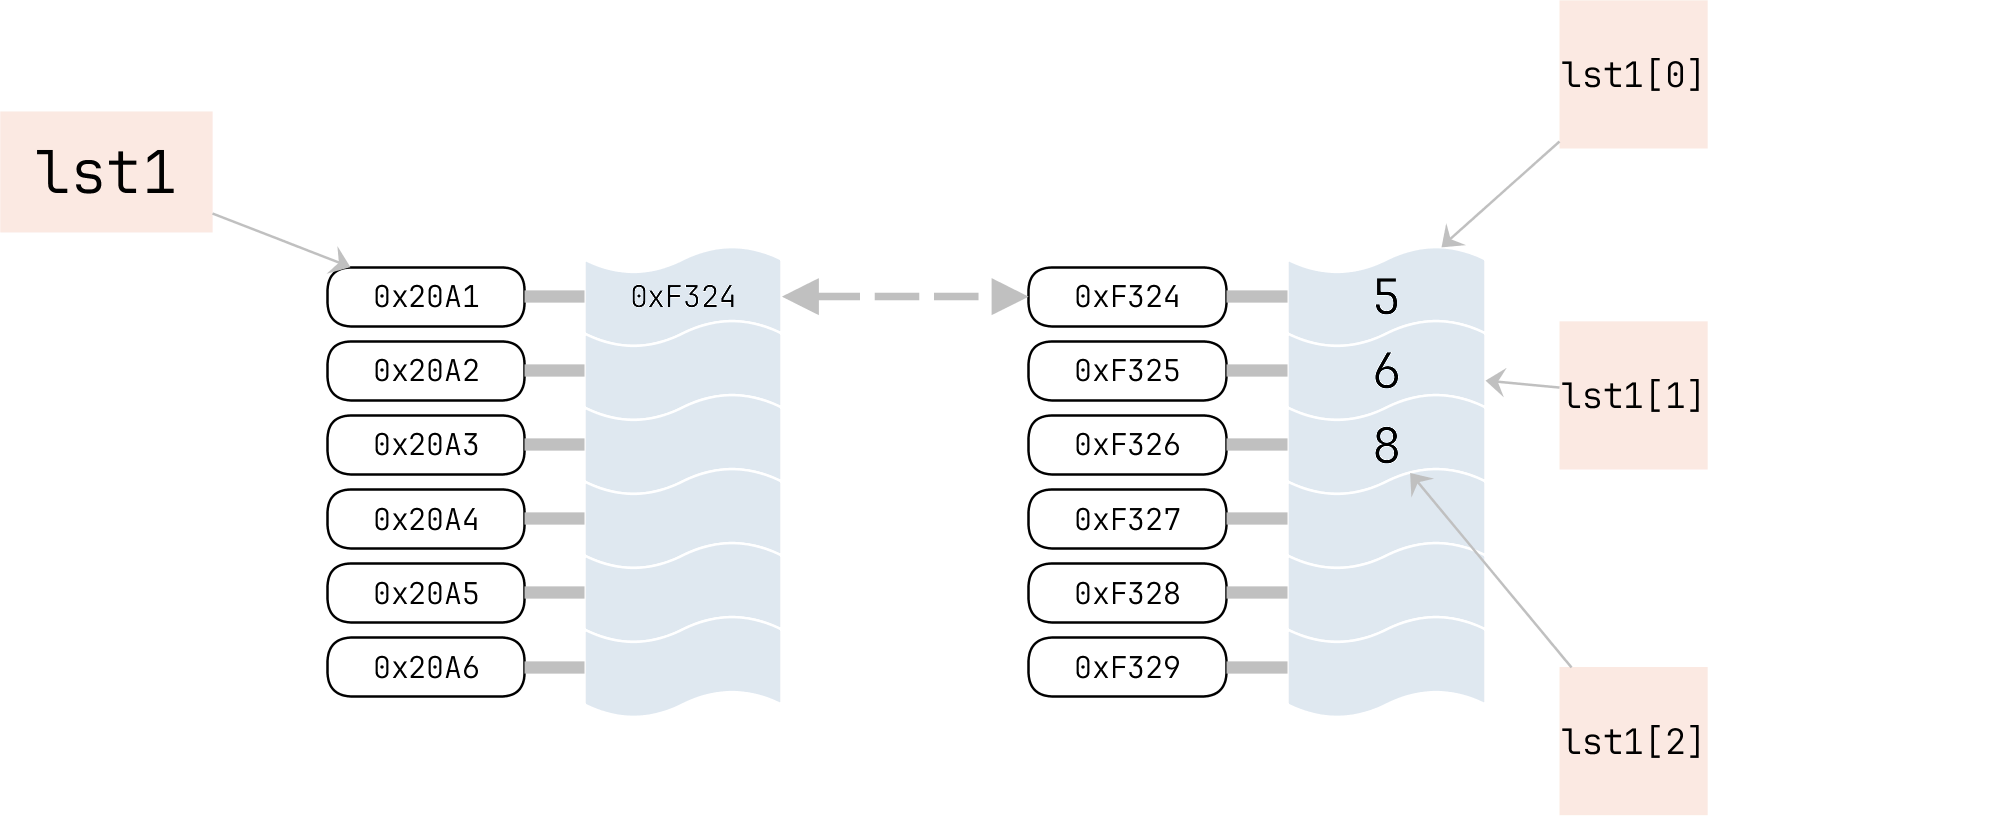
\includegraphics[width=\linewidth]{ch-listes/img/mut1.png}\\


\mintinline{python}{lst2 = lst1}\\

La variable \mintinline{python}{lst2} est associée à la même valeur que \mintinline{python}{lst1}.\\
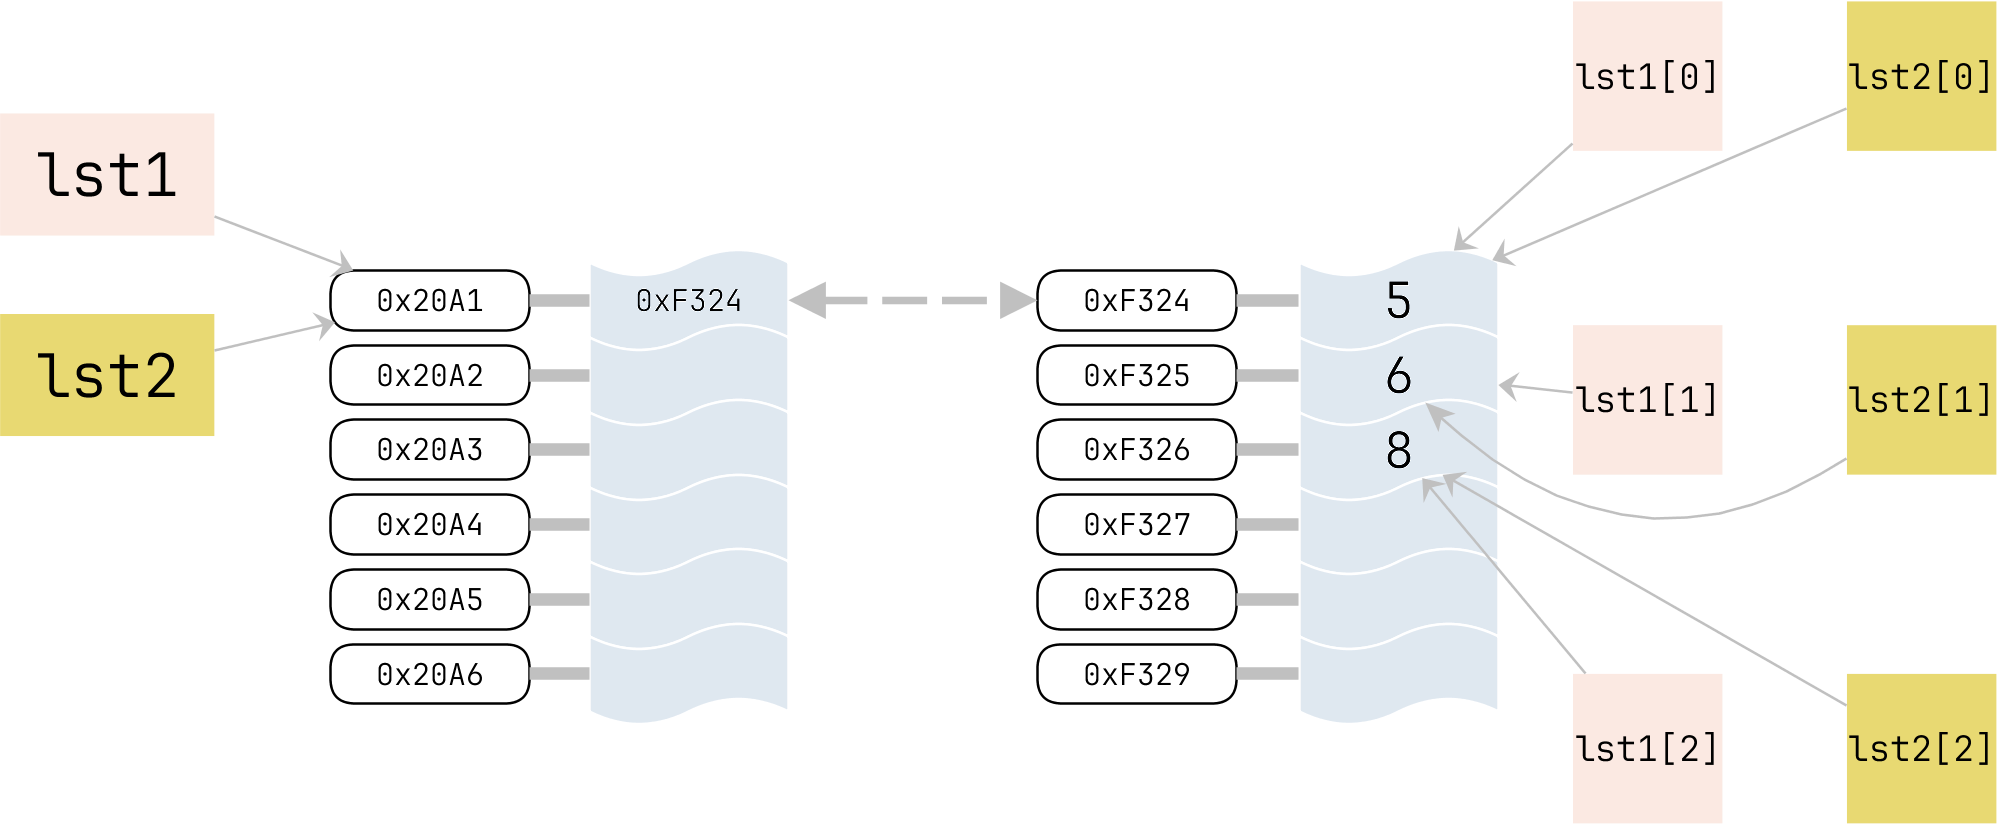
\includegraphics[width=\linewidth]{ch-listes/img/mut2.png}\\


\mintinline{python}{lst1[0] = 10}\\

La valeur de \mintinline{python}{lst1[0]} est changée, elle l'est donc aussi pour \mintinline{python}{lst2}.\\
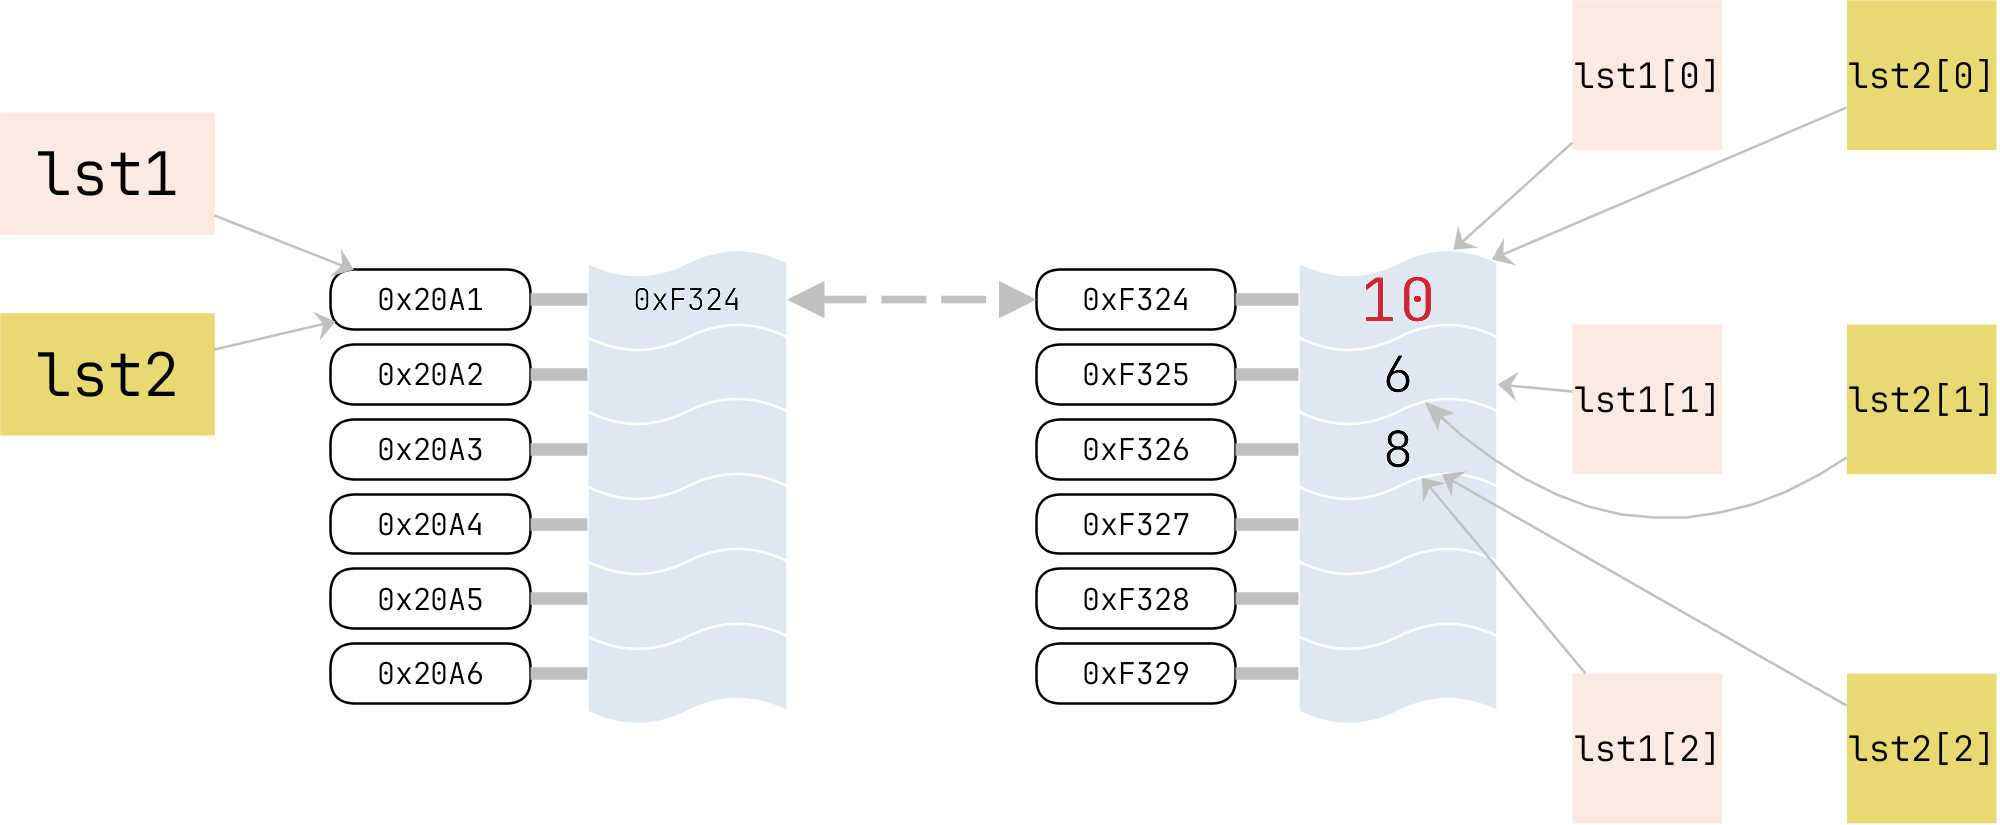
\includegraphics[width=\linewidth]{ch-listes/img/mut3.png} \\
Voilà donc pourquoi lorsqu'on écrit \mintinline{python}{lst2 = lst1}, tout changement dans \mintinline{python}{lst1} se reflète aussi dans \mintinline{python}{lst2} et vice-versa.\\

\subsubsection{Copier une liste (bonne méthode)}



\mintinline{python}{lst2 = lst1[:]}\\

Les éléments de \mintinline{python}{lst1} sont recopiés dans une autre zone mémoire, et \mintinline{python}{lst2} « pointe » sur l'adresse du début de cette zone.\\
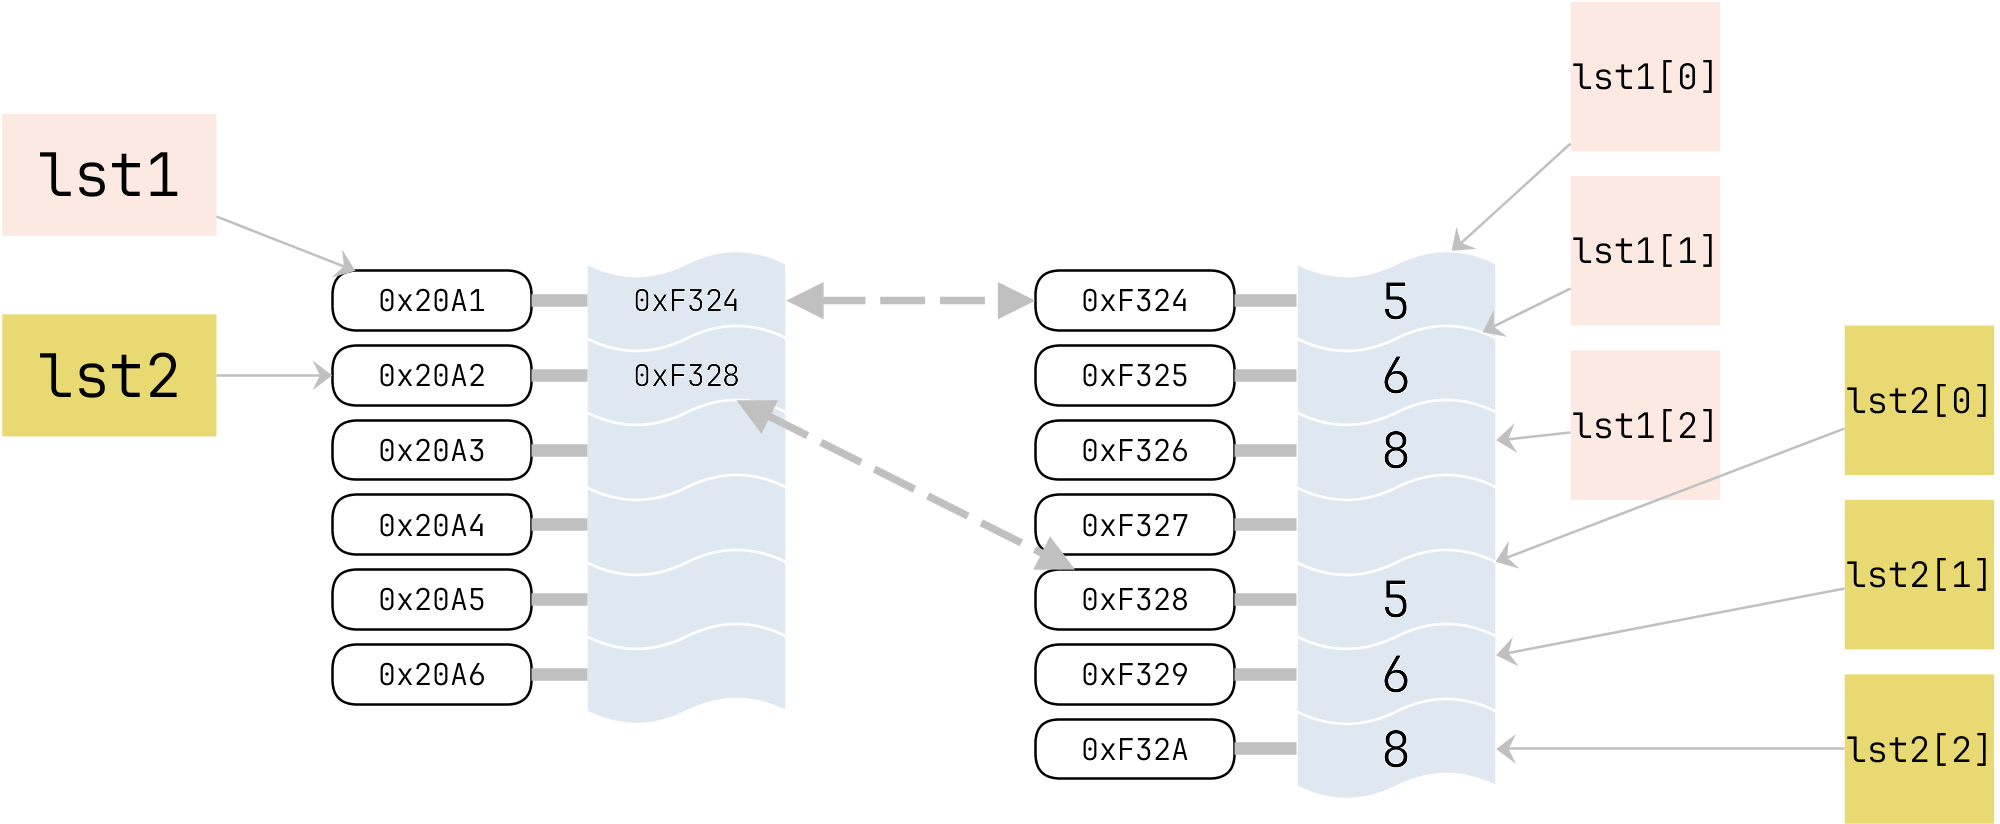
\includegraphics[width=\linewidth]{ch-listes/img/mut4.png}\\


\mintinline{python}{lst1[0] = 10}\\

Le changement n'affecte pas \mintinline{python}{lst2}.\\
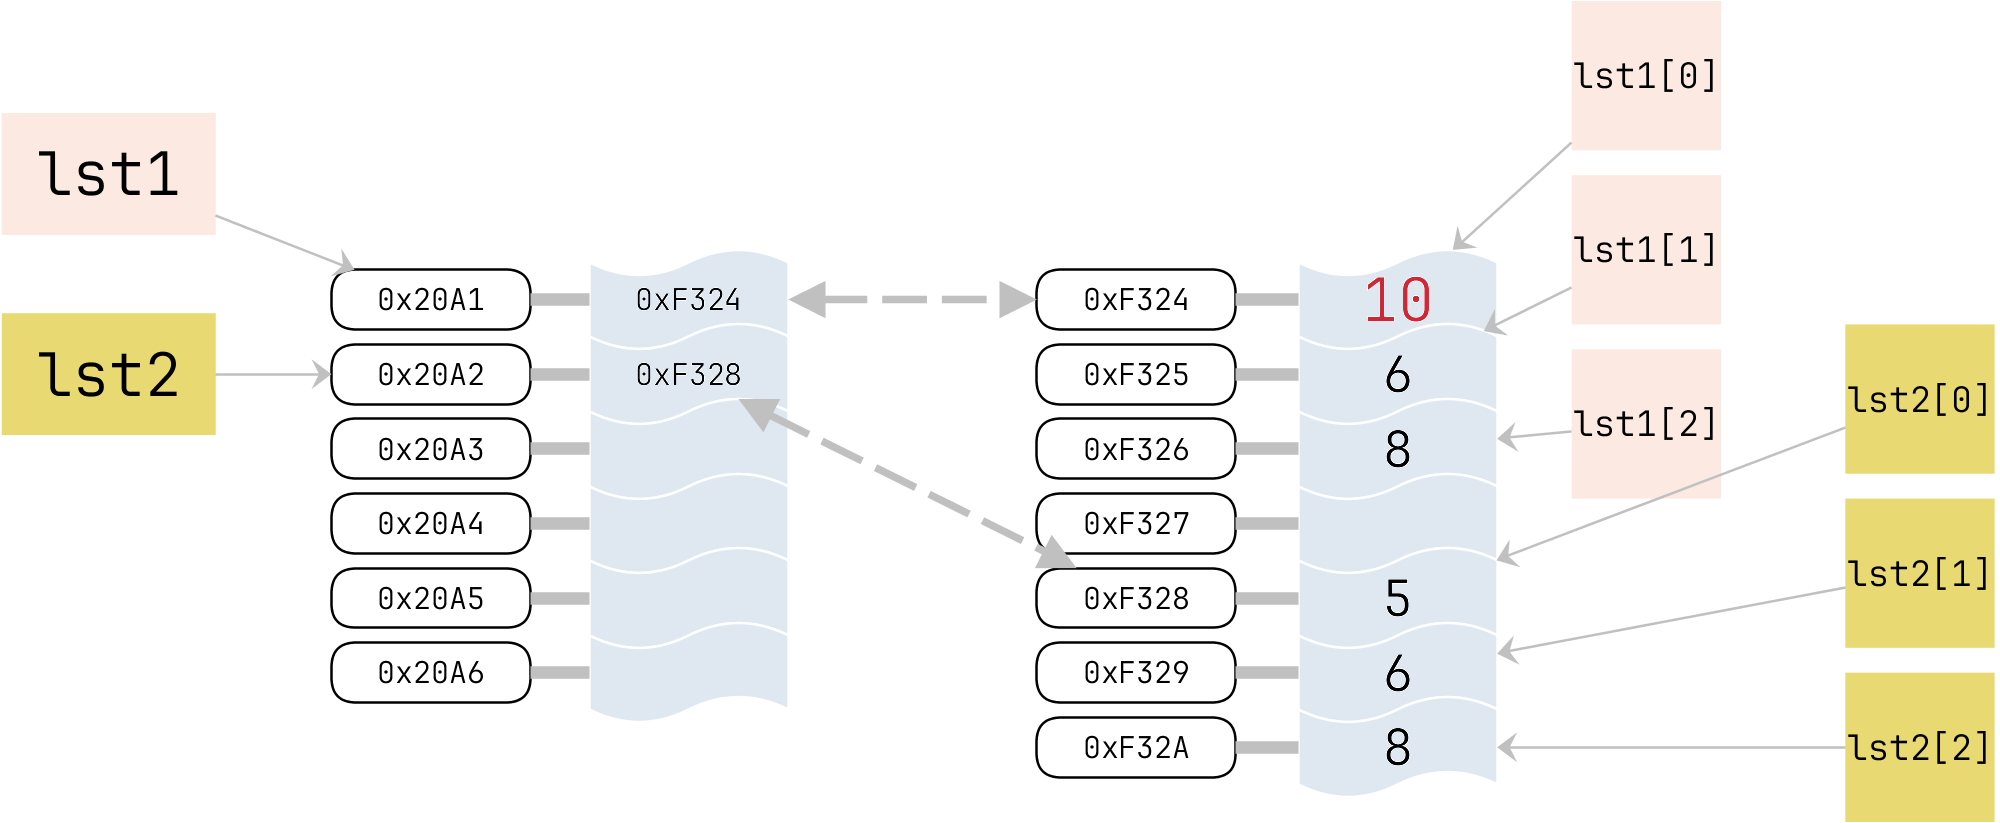
\includegraphics[width=\linewidth]{ch-listes/img/mut5.png}